% ─────────────────────────────────────────────────────────────────
\section{Analysis and Discussion}
\label{sec:discussion}
% ─────────────────────────────────────────────────────────────────

\subsection{Confusion Pairs: Architecture-Limited, Not Data-Limited}
\label{sec:discussion:confusion}

The class pairs (61,\,90) and (70,\,56) generate incorrect predictions in
\textit{every HierGIN configuration} we tested, as well as in Mamba3D and
PointMamba.
We initially attributed this to data-intrinsic near-inseparability.
\textbf{This conclusion was premature.}

RIConv2 RUN1 --- using \emph{only} xyz coordinates and surface normals, no
electrostatic potential --- achieves F1\,=\,0.887 on class\,61 and
F1\,=\,0.967 on class\,90, with only 13 cross-confusions between them
(vs.\ HierGIN-8D's F1\,=\,0.576/0.850 with all features).
The full per-class comparison is in Table~\ref{tab:per_class_riconv}.

\begin{table}[h]
  \centering
  \caption{Per-class F1 on the seven hardest classes.
           RIConv2 geometry-only (RUN1) dramatically outperforms HierGIN-8D
           on every hard class, despite using no chemical features.
           This refutes the claim that (61,90) confusion is data-intrinsic.}
  \label{tab:per_class_riconv}
  \begin{tabular}{lrrrrrrr}
    \toprule
    \textbf{Method} & \textbf{cls\,61} & \textbf{cls\,90} & \textbf{cls\,70}
      & \textbf{cls\,56} & \textbf{cls\,86} & \textbf{cls\,14} & \textbf{cls\,80} \\
    \midrule
    HierGIN-8D (all feats)     & 0.576 & 0.850 & 0.532 & 0.775 & 0.667 & 0.729 & 0.174 \\
    HierGIN-14D (global norm)  & ---   & ---   & ---   & ---   & ---   & ---   & ---   \\
    \midrule
    RIConv2 RUN1 (geom only)   & 0.887 & 0.967 & 0.708 & 0.879 & 0.722 & 0.820 & 0.240 \\
    RIConv2 RUN2 (geom+Pot)    & 0.914 & 0.977 & 0.708 & 0.901 & 0.812 & 0.864 & 0.222 \\
    \bottomrule
  \end{tabular}
\end{table}

The confusion is \textbf{architecture-limited}, not data-limited.
Our separability analysis (Section~\ref{sec:analysis:ri}) correctly showed
that single-scale marginal distributions of edge-level RI scalars
(KS\,$\leq$0.004 for pair 61/90) are near-identical.
But this measures the wrong geometric representation: RIConv2 does not
classify on single edge scalars --- it builds multi-scale rotation-invariant
local patch descriptors via ball-query grouping at four radius scales,
enabling it to encode local surface shape that is invisible to a kNN-6 graph.
The separability analysis was thus not wrong; it correctly characterised what
\textit{HierGIN} can access, not what the data contains.

The revised \textbf{theoretical macro-F1 ceiling} is substantially higher than
our earlier estimate of 0.85--0.88.
RIConv2 RUN2 achieves 0.854; class\,80 (only 14 test samples, F1\,=\,0.24) is
the remaining hard constraint.
A perfect classifier on classes 1--79,81--99 with RIConv2-level performance on
class\,80 would approach macro-F1\,$\approx$\,0.95.

\subsection{Feature Role Summary}

Table~\ref{tab:feature_roles} synthesises the role of each feature group.
We now distinguish \textit{within-HierGIN} impact (from our ablation) from
\textit{cross-architecture} evidence (from RIConv2).

\begin{table}[h]
  \centering
  \caption{Feature group roles. ``HierGIN impact'' = ablation delta.
           ``Cross-arch'' = what RIConv2 reveals about the signal when
           extracted by a stronger architecture.}
  \label{tab:feature_roles}
  \begin{tabular}{lp{2.6cm}p{5.8cm}}
    \toprule
    \textbf{Feature} & \textbf{HierGIN impact} & \textbf{Interpretation} \\
    \midrule
    Potential & $-$11.8\,pp if removed & Dominant within HierGIN; KS / SW confirm
      large distributional differences for most pairs.
      Cross-arch: adds only $+$1.6\,pp over RIConv2 geometry-only (0.838→0.854),
      suggesting geometry is the primary signal when properly extracted. \\[4pt]
    NormalPotential & $-$0.9\,pp overall; $-$14\,pp cls\,61 & Secondary chemical
      signal; critical for (61,\,90) within HierGIN. \\[4pt]
    Normals (surface) & $-$3.2\,pp (4D$\to$8D) within HierGIN &
      Cross-arch: geometry-only RIConv2 using normals + xyz achieves 0.838
      macro-F1 --- normals are the \emph{primary} signal for a rotation-invariant
      multi-scale architecture. \\[4pt]
    Coordinates & Necessary context for GNN aggregation & Cross-arch: RIConv2
      ball-query grouping exploits coordinates to define local reference frames
      and multi-scale patches. \\[4pt]
    Multi-scale local geometry & Not available to HierGIN & RIConv2 RUN1 result
      shows this is worth $+$21.9\,pp macro-F1 over HierGIN-6D (0.619),
      dwarfing any single-feature ablation within HierGIN. \\
    \bottomrule
  \end{tabular}
\end{table}

\subsection{Hierarchical vs.\ Flat GNN}

The hierarchical two-level pooling consistently outperforms a flat 6-layer GIN
by $+$15.8\,pp macro-F1 (0.798 vs.\ 0.640).
We attribute this gap to two factors:

\paragraph{Spatial hierarchy.}
The Voronoi patch pooling creates a mid-scale representation that captures
local surface regions (e.g., a charged patch, a concave groove) as single
patch nodes.
The patch-level GIN can then reason about the spatial arrangement of these
regions, a capability absent in a flat single-level GNN with global pooling.

\paragraph{Information bottleneck.}
Compressing 1\,000 nodes to 64 patches before global readout acts as a
structured pooling bottleneck, reducing the variance of the graph embedding
and improving generalisation under the heavy class imbalance.

\subsection{Why RIConv2 Dominates: Architecture, Not Features}
\label{sec:discussion:riconv2}

The 3\,pp gap between RIConv2 RUN1 (geometry-only, macro-F1\,=\,0.838) and
our best HierGIN model (all 14D features, 0.808) is explained by two
architectural differences.

\paragraph{Multi-scale ball-query grouping vs.\ single-scale kNN.}
RIConv2 uses four set-abstraction layers, each grouping points within a fixed
radius ball at a different scale and aggregating RI-invariant messages within
the group.
This produces hierarchical local shape descriptors: scale-1 captures small
surface bumps and grooves; scale-4 captures the overall protein curvature profile.
HierGIN's kNN-6 graph connects each node to its 6 nearest neighbours at a
single fixed scale; the Voronoi pooling then collapses 1\,000 nodes to 64
patches.
This two-level hierarchy is coarser and scale-rigid --- it cannot simultaneously
reason about local curvature and global shape the way RIConv2's four-scale
aggregation does.

\paragraph{RI features within groups vs.\ on graph edges.}
Our RI-GIN computes 5 invariant scalars on each kNN-6 graph edge.
RIConv2 computes the same scalars between a centre point and every member of
its local ball-query group, then applies a shared MLP and aggregates.
Because the group radius is fixed in 3D, all members of a group share a common
geometric context --- they lie on the same local surface patch.
The 5 scalars computed within such a group encode the local normal variation,
curvature direction, and surface smoothness of that patch, not just the pairwise
geometry of two distant neighbours.
This is why our separability analysis (SW(RI)\,=\,0.004 for pair 61/90) correctly
showed no separability for kNN-6 edge-level distributions, yet RIConv2 geometry-only
achieves F1\,=\,0.887 on class\,61: the discriminating signal lives in
multi-scale local patch geometry, not in the marginal distribution of individual
edges.

\paragraph{Conclusion.}
The pair (61,\,90) is separable from surface geometry.
HierGIN could not exploit this because its kNN-6 graph and single-scale Voronoi
pooling are too coarse to capture the relevant geometric signal.
The path forward is adopting or integrating RIConv2-style multi-scale local
grouping, not adding more chemical features.

\subsection{Why Point-cloud Methods Underperform}

Mamba3D (0.672) and PointMamba (0.720) process the protein as a 3D point cloud
but use generic sequence-based or Mamba-block architectures without surface-mesh
topology or rotation-invariant local convolution.
Despite expressive backbones, they trail RIConv2's geometry-only model by
17\,pp (0.838 vs.\ 0.720), confirming that surface-topology awareness
\emph{and} rotation-invariant local convolution together drive performance,
not just model capacity.

\subsection{What Could Push Beyond the Current Ceiling}

RIConv2 RUN2 at macro-F1\,=\,0.854 is now the benchmark to beat.
Class\,80 (14 test samples, F1\,=\,0.222--0.240 for all methods) remains the
primary hard constraint given extreme data scarcity.
Directions most likely to yield further gains:

\begin{itemize}
  \item \textbf{Multi-scale RI architecture in a hierarchical GNN.}
        Replacing HierGIN's kNN-6 node stage with RIConv2-style ball-query
        multi-scale grouping while retaining the Voronoi patch-level GNN
        would combine the best of both: multi-scale local geometry extraction
        and coarse-level spatial reasoning.
        This is the highest-priority direction given that the architecture gap
        (3\,pp) exceeds any feature engineering gain we found.

  \item \textbf{Chemical features on a strong geometric backbone.}
        RIConv2 RUN2 shows that adding Potential to geometry gives
        $+$1.6\,pp (0.838$\to$0.854).
        Applying the full 8D or 14D feature set within a RIConv2-style
        architecture would combine both advantages.

  \item \textbf{Addressing class\,80 with few-shot techniques.}
        Class\,80 is predicted as 70 or 56 by all methods (7--8 out of 14
        test samples).
        Prototypical or metric-learning approaches that do not require many
        training examples could improve rare-class recall.

  \item \textbf{Sequence features}: ESM-2 embeddings~\cite{esm2} would add
        fold-family information not visible on the surface --- the only signal
        that could help for families whose surfaces are truly chemically and
        geometrically similar.

  \item \textbf{Contrastive pre-training} on full-resolution VTK meshes
        ($\approx$10\,676 vertices) to learn richer node representations
        before FPS subsampling.
\end{itemize}

\subsection{Why RI-GIN Improves over Standard GIN}
\label{sec:analysis:ri_sep}

Section~\ref{sec:analysis:ri} showed that the five SO(3)-invariant RI edge
scalars have universally lower Sliced Wasserstein distances than the 8D node
features for confusable pairs (SW(RI)\,$\leq$\,0.006 vs SW(8D)\,=\,0.027--0.140),
and KS values near zero for all confusable pairs ($\leq$0.041, vs Potential
KS\,=\,0.031--0.250).
This rules out the possibility that RI-GIN gains its improvement
($+$0.2\,pp macro-F1, $+$1.3\,pp balanced accuracy over standard GIN)
by accessing richer geometric information.

\begin{figure}[h]
  \centering
  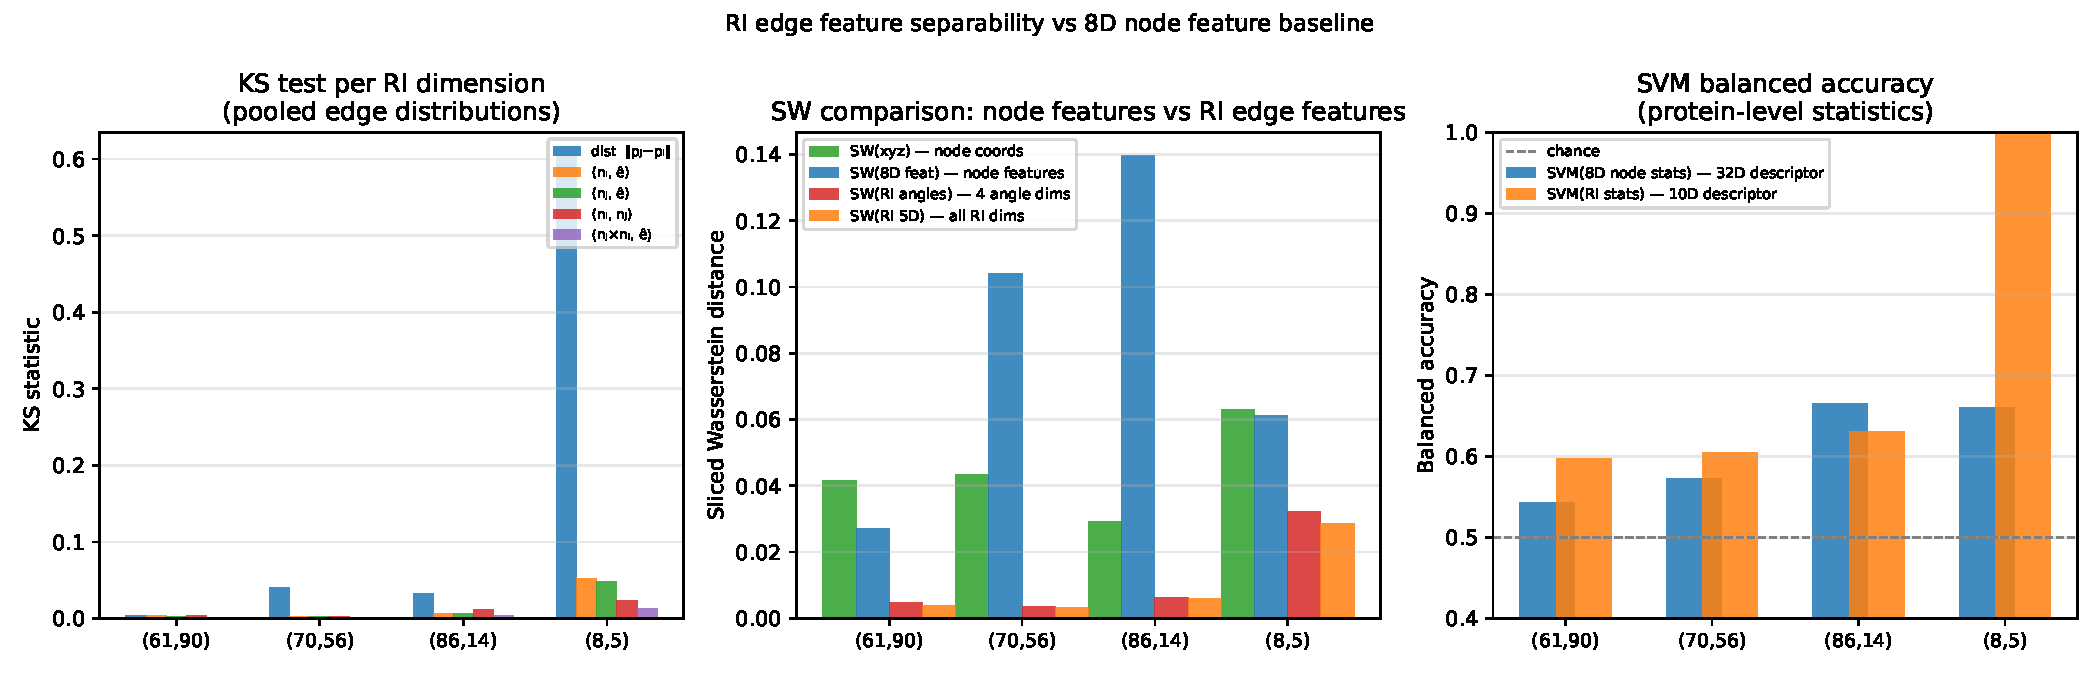
\includegraphics[width=\textwidth]{figures/separability_ri_features.pdf}
  \caption{RI edge feature separability analysis (full data in
           Tables~\ref{tab:ks_ri}--\ref{tab:svm_ri}).
           \textbf{Left:} KS statistic per RI dimension — confusable pairs
           (top three) are near zero across all dimensions; only the control
           (8,5) separates cleanly via edge length (KS\,=\,0.605).
           \textbf{Middle:} SW(RI 5D) is 7--23$\times$ lower than
           SW(8D node feat) for confusable pairs.
           \textbf{Right:} SVM balanced accuracy (5-fold CV) — RI protein
           statistics match or slightly exceed 8D for (61,90) and (70,56),
           but (86,14) remains better separated by electrostatics.}
  \label{fig:ri_sep}
\end{figure}

The improvement from RI-GIN is therefore a \textbf{representation effect}
rather than a feature-enrichment effect.
Hard-coding rotation invariance into the edge message function removes the
burden of learning approximate invariance from data, producing embeddings
that are more consistent across proteins regardless of their orientation in
global coordinates.
This acts as a form of geometric regularisation: the model wastes fewer
parameters on orientation-specific patterns and more on the discriminating
chemistry.

A secondary contribution comes from the global shape signal captured in RI
edge-length statistics: per-protein mean edge length correlates with protein
size, providing an orthogonal, size-encoded representation that slightly boosts
SVM balanced accuracy for (61,\,90) ($+$5\,pp) and (70,\,56) ($+$3\,pp) over
the 8D node-feature baseline.
This cross-protein scale information is naturally present in the RI distance
dimension without any special normalisation, unlike the geometric features
which required explicit global normalisation to prevent per-protein z-scoring
from erasing it.

\subsection{Limitations}

\begin{itemize}
  \item Our analysis uses a fixed FPS seed; results may vary slightly with
        different subsampling seeds, especially for very small proteins.
  \item The PNA backbone could not be evaluated with the proper inference
        protocol due to a missing training-time delta parameter; its test
        metrics are a lower bound.
  \item The VTK mesh showcase (Figure~\ref{fig:vtk}) uses 3D matplotlib
        rendering with triangle subsampling for visual clarity; the actual
        mesh is finer.
  \item We evaluate on the SHREC\,25 train/test split; cross-dataset
        generalisation to other protein family benchmarks is not assessed.
\end{itemize}
